%! TEX root = main.tex

\graphicspath{{00_Images/10_chapter/}}

\chapter{Electronic Noise}
\label{ch:noise}

\section{Noise Definition and Modeling}
\label{sc:101}

Electronic noise is the random, unpredictable fluctuation of voltage or current that every real device superimposes on the signal it processes.
Unlike a deterministic disturbance such as the \SI{50}{\hertz} hum picked up from the mains supply, noise is intrinsic to the physics of the components and cannot be filtered out by tuning to a single frequency, so a complete signal at a node is written as the sum
\[
v(t) = V_{DC} + v_s(t) + v_n(t) + v_d(t)
\]
where \(V_{DC}\) is the bias, \(v_s(t)\) the wanted signal, \(v_n(t)\) the random noise, and \(v_d(t)\) the deterministic disturbance.
Random noise has zero mean, \(\overline{v_n} = 0\), so its strength is measured not by its average but by its root-mean-square value, which is proportional to the square root of its power:
\[
v_{n,RMS} = \sqrt{\lim_{T \to \infty} \frac{1}{T}\int_0^T v_n^2(t) dt}
\]
The quality of a signal is then quantified by the signal-to-noise ratio, the ratio of the wanted to the unwanted root-mean-square amplitude, usually expressed in decibels:
\[
\mathrm{SNR} = \frac{v_{s,RMS}}{v_{n,RMS}}, \qquad \mathrm{SNR}_{dB} = 20\log_{10}\mathrm{SNR}
\]

\subsection{Noise Power Spectral Density}
\label{ssc:1011}

Because noise is spread over frequency, the natural description is its power spectral density, the noise power per unit bandwidth, taken with voltage or with current as reference:
\[
S_{n,V} = \frac{d\overline{v_n^2}}{df}\quad\left[\frac{\mathrm{V}^2}{\mathrm{Hz}}\right], \qquad S_{n,I} = \frac{d\overline{i_n^2}}{df}\quad\left[\frac{\mathrm{A}^2}{\mathrm{Hz}}\right]
\]
Integrating the density over the bandwidth of interest recovers the mean-square value, and hence the root-mean-square amplitude:
\[
\int_{BW} S_{n,V}(f) df = \overline{v_n^2} = v_{n,RMS}^2
\]
Two spectral shapes dominate in practice.
White noise has a flat density, constant across the spectrum, while flicker noise, also called pink or \(1/f\) noise, has a density that falls inversely with frequency and therefore concentrates its power at the low end of the band.
Since the audio range is, in electronic terms, a low-frequency range, flicker noise is particularly relevant in audio circuits, and a real device shows a \(1/f\) region at low frequency that flattens into a white region above a transition frequency, as illustrated in figure \ref{fig:npsdShape}.

\begin{figure}[!htb]
    \centering
    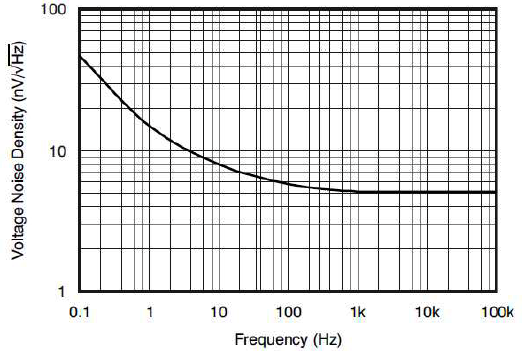
\includegraphics[width=0.55\textwidth]{Input_Voltage_Noise_Density.png}
    \caption{Typical input voltage noise density of a device: a \(1/f\) flicker region at low frequency flattening into a white-noise plateau above the corner frequency}
    \label{fig:npsdShape}
\end{figure}

When such a noise density passes through a linear stage of transfer function \(TF(j\omega)\), it is shaped exactly as a signal power would be, by the squared magnitude of the transfer function:
\[
S_{out,n} = |TF(j\omega)|^2  S_{in,n}
\]

\subsection{The Two-Generator Model}
\label{ssc:1012}

A real two-port device adds noise that cannot be captured by a single source, because the noise it injects depends on how the input is terminated.
The standard equivalent model therefore places two noise generators at the input: a voltage noise generator \(v_n\) in series with the input, and a current noise generator \(i_n\) in parallel with it.

\begin{figure}[!htb]
    \centering
    \subfloat[Short-circuited input: \(i_n\) is shunted to ground and only \(v_n\) is measured]{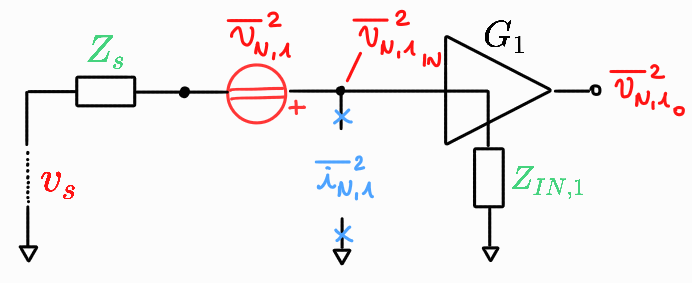
\includegraphics[height=0.13\textheight]{Voltage_Component.png}}
    \hfill
    \subfloat[Open or high-impedance input: \(i_n\) flows through the input impedance, producing \(i_n Z_{in}\)]{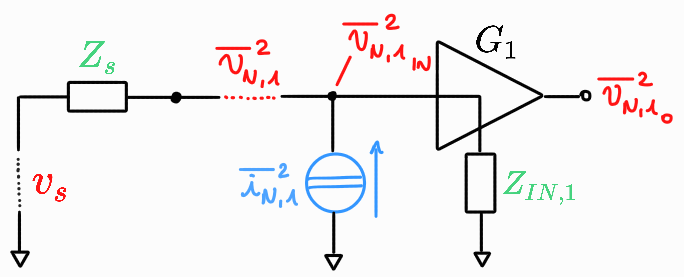
\includegraphics[height=0.13\textheight]{Current_Component.png}}
    \caption{The two-generator noise model and the two limiting measurements that isolate each contribution}
    \label{fig:twoGenerators}
\end{figure}

The need for both generators is revealed by two limiting measurements, shown in figure \ref{fig:twoGenerators}.
When the input is short-circuited, the parallel current generator is shunted to ground and contributes nothing, so the output noise is due entirely to the series voltage generator \(v_n\).
When the input is left open, or terminated on a high impedance, the series voltage generator finds no path while the current generator drives the input impedance, so the measured noise reflects \(i_n\) multiplied by the input impedance.
The two measurements separate and quantify the voltage and current contributions, and they already foreshadow the central design lesson: the current generator becomes important only when the source impedance is high.

\section{Noise in Multi-Stage Systems}
\label{sc:102}

In a chain of amplifying stages the wanted signal is multiplied by every gain in turn, but the noise of each stage enters at a different point and is amplified only by the stages that follow it.

\begin{figure}[!htb]
    \centering
    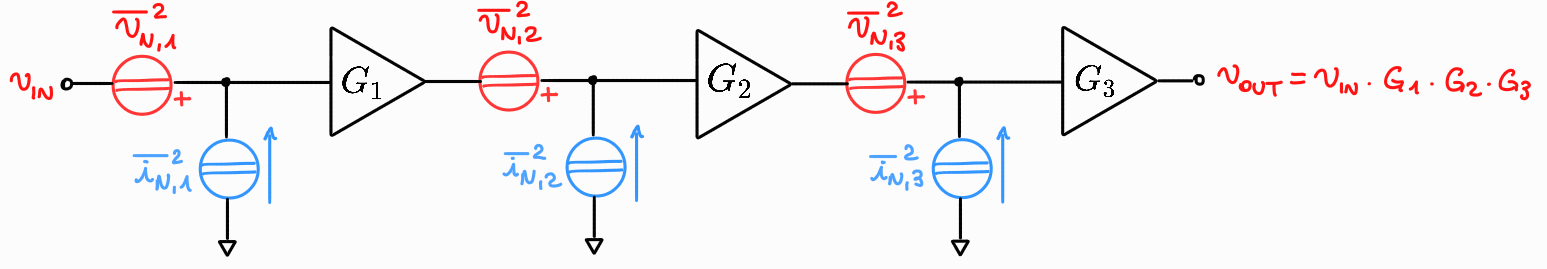
\includegraphics[width=0.80\textwidth]{Multi_Stage_Noise_Pipeline.png}
    \caption{Cascade of three noisy stages, each contributing its own input-referred noise density \(S_{N,i}\) and gain \(G_i\)}
    \label{fig:multiStageNoise}
\end{figure}

For the three-stage cascade of figure \ref{fig:multiStageNoise}, where stage \(i\) has input-referred noise density \(S_{N,i}\) and transfer function \(TF_i\), the noise contributions add in power at the output:
\[
S_{out,N} = S_{N,1}|TF_1  TF_2  TF_3|^2 + S_{N,2}|TF_2  TF_3|^2 + S_{N,3}|TF_3|^2
\]
The signal at the output is \(v_{s,RMS}|TF_1  TF_2  TF_3|\), so referring the noise back to the input, by dividing each contribution by the gain that precedes it, gives the signal-to-noise ratio
\[
\mathrm{SNR} = \frac{v_{s,RMS}}{\sqrt{\displaystyle\int_{BW}\left(S_{N,1} + \frac{S_{N,2}}{|TF_1|^2} + \frac{S_{N,3}}{|TF_1  TF_2|^2}\right)df}}
\]
The structure of this expression carries the most important result of the whole chapter.
The noise of the first stage enters undivided, while the noise of every later stage is divided by the gain of all the stages preceding it, so a large first-stage gain makes the later contributions negligible.

\paragraph{The golden rule of low-noise design} The first stage, the preamplifier, must combine the lowest possible noise with the highest possible gain.
A high first-stage gain \(G_1\) drives the terms \(S_{N,2}/|TF_1|^2\) and \(S_{N,3}/|TF_1  TF_2|^2\) toward zero, so that in the limit \(G_1 \to \infty\) the overall signal-to-noise ratio is set by the first stage alone:
\[
\mathrm{SNR}_{max} = \frac{v_{s,RMS}}{\sqrt{\displaystyle\int_{BW} S_{N,1} df}}
\]
This is the fundamental reason why the preamplifier is the most critical component of any audio chain, and why its noise specification, established before any further amplification, determines the achievable dynamic range of the entire system.

\section{Noise in Components}
\label{sc:103}

The input-referred noise densities used above originate in the elementary physical mechanisms of the individual components, which fall into two families: thermal noise, tied to temperature, and shot noise, tied to bias current.

\subsection{Resistors: Thermal Noise}
\label{ssc:1031}

Inside any resistor the charge carriers are in perpetual random thermal motion, and this agitation produces a fluctuating voltage across the terminals even with no applied bias.
This is thermal noise, also called Johnson noise, and its voltage power spectral density is
\[
S_{n,V}^{R} = 4 k_B T R
\]
where \(k_B = \SI{1.38e-23}{\joule\per\kelvin}\) is the Boltzmann constant, \(T\) the absolute temperature, and \(R\) the resistance.
The density is independent of frequency, so thermal noise is a white process, and the root-mean-square voltage over a bandwidth \(BW\) is
\[
v_{n,RMS} = \sqrt{\int_{BW} 4 k_B T R df} = \sqrt{BW \cdot 4 k_B T R}
\]

For a \SI{1}{\kilo\ohm} resistor at \(T = \SI{300}{\kelvin}\), the density is \(S_{n,V}^{R} \approx \SI{1.66e-17}{\volt\squared\per\hertz}\), and integrating over the audio band from \SI{20}{\hertz} to \SI{20}{\kilo\hertz} gives a root-mean-square noise of roughly \SI{0.57}{\micro\volt}.
Applying Ohm's law converts the voltage density into the equivalent current density seen when the resistor is viewed as a noise current source:
\[
S_{n,I}^{R} = \frac{S_{n,V}^{R}}{R^2} = \frac{4 k_B T R}{R^2} = \frac{4 k_B T}{R}
\]

\subsection{PN Junctions: Shot Noise}
\label{ssc:1032}

When a current crosses a potential barrier, such as a pn junction, it is carried by discrete electrons that arrive at random instants rather than as a perfectly smooth flow.
The granularity of this charge transport produces a fluctuation called shot noise, whose current power spectral density is proportional to the bias current:
\[
S_{n,I} = 2 q I
\]
where \(q = \SI{1.6e-19}{\coulomb}\) is the electron charge and \(I\) the current through the junction.
Like thermal noise, shot noise is white, but it differs in a fundamental way that is summarized in table \ref{tab:thermalVsShot}.

\begin{figure}[!htb]
    \centering
    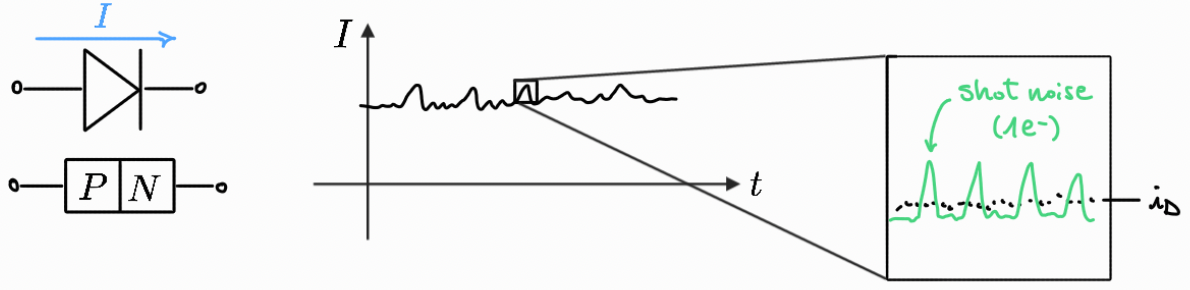
\includegraphics[width=0.70\textwidth]{shot_noise.png}
    \caption{Shot noise arises from the discrete arrival of charge carriers crossing the junction, giving a current fluctuation proportional to the bias current}
    \label{fig:shotNoise}
\end{figure}

\begin{table}[!htb]
\centering
\renewcommand{\arraystretch}{1.3}
\begin{tabular}{c|c}
\hline
\textbf{Thermal noise} & \textbf{Shot noise} \\
\hline
Set by the resistance and the material & Set by the bias current \\
Depends on temperature & Independent of temperature \\
Reducible by cooling & Does not depend on the material \\
\hline
\end{tabular}
\caption{Comparison of the two white-noise mechanisms}
\label{tab:thermalVsShot}
\end{table}

\subsection{Transistors}
\label{ssc:1033}

The noise of a transistor follows directly from these two mechanisms, applied to the device of chapter \ref{ch:transistors}, and the difference between bipolar and field-effect devices is decisive for audio.

For the bipolar junction transistor the dominant contribution is the shot noise of the collector current, a current noise whose density is
\[
S_{n,I}^{BJT} = 2 q I_C
\]
which, referred to the input through the transconductance, gives an equivalent voltage noise density
\[
S_{n,V}^{BJT} = \frac{2 q I_C}{g_m^2}
\]

For field-effect devices the gate draws essentially no current, with \(I_G\) of the order of picoamperes for the JFET and femtoamperes for the MOSFET, so the input current noise \(S_{n,I} = 2 q I_G\) is negligible.
The relevant mechanism is instead the thermal noise of the conducting channel, modeled as the thermal noise of an equivalent resistance \(1/g_m\):
\[
S_{n,I}^{FET} = 4 k_B T g_m \quad \Rightarrow \quad S_{n,V}^{FET} = \frac{4 k_B T g_m}{g_m^2} = \frac{4 k_B T}{g_m}
\]

\begin{figure}[!htb]
    \centering
    \subfloat[Noise model of the BJT: dominant collector shot-noise current]{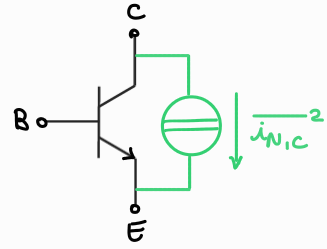
\includegraphics[height=0.18\textheight]{BJT_Noise.png}}
    \hspace{1.5cm}
    \subfloat[Noise model of the JFET and MOSFET: negligible gate current noise, thermal channel noise]{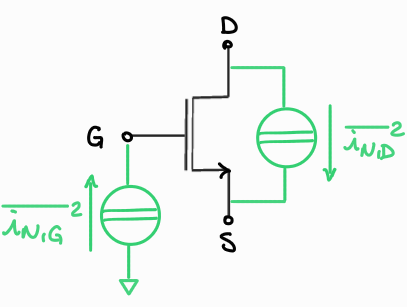
\includegraphics[height=0.18\textheight]{JFET_MOSFET_Noise.png}}
    \caption{Input noise models of the bipolar and field-effect transistors}
    \label{fig:transistorNoise}
\end{figure}

The flicker and white regions of these devices meet at a corner frequency, below which \(1/f\) noise dominates.
For the BJT and the JFET this corner lies around \SI{10}{\hertz}, comfortably below the audio band, whereas for the MOSFET it sits much higher, often above the audio range, which makes the MOSFET a poor choice for low-noise audio despite its dominance in integrated circuits, where its small size and high integration density prevail.

\begin{figure}[!htb]
    \centering
    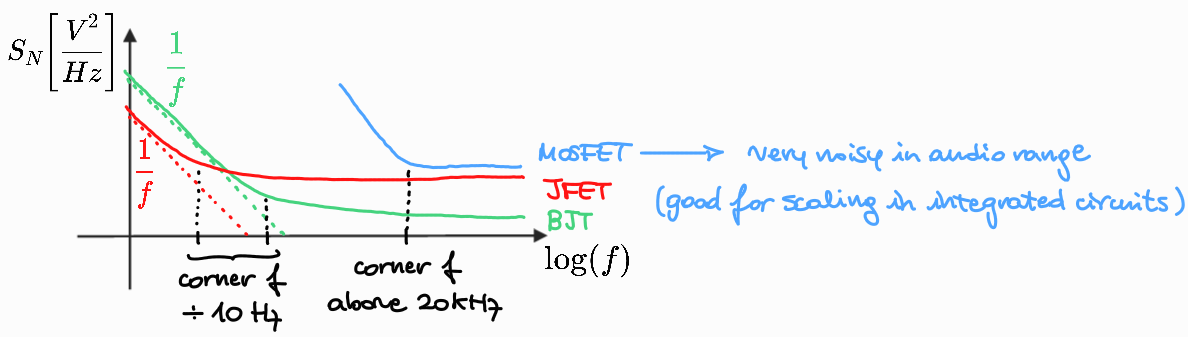
\includegraphics[width=0.70\textwidth]{Corner_Frequency.png}
    \caption{Noise power spectral density of a transistor: the \(1/f\) and white asymptotes meet at the corner frequency}
    \label{fig:cornerFreq}
\end{figure}

\section{Design Choice: BJT versus FET}
\label{sc:104}

The choice between a bipolar and a field-effect input stage is governed almost entirely by the impedance of the source that drives it.
The total input-referred noise gathers the voltage noise of the device, the current noise flowing through the source resistance, and the thermal noise of the source itself:
\[
v_{n,tot} = \sqrt{v_n^2 + (i_n R_S)^2 + 4 k_B T R_S}
\]
The middle term, the voltage developed by the device current noise across the source resistance, scales directly with \(R_S\), and it is this term that separates the two technologies.

\begin{figure}[!htb]
    \centering
    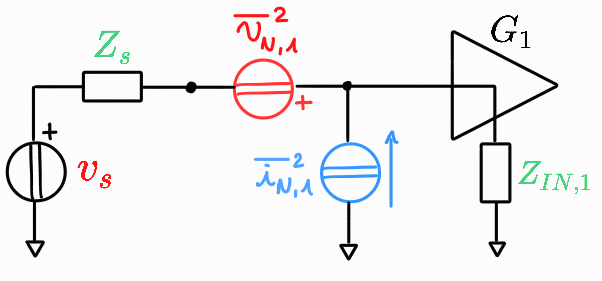
\includegraphics[width=0.45\textwidth]{Source_Impedance_Noise.png}
    \caption{The source impedance converts the input current noise into a voltage noise \(i_n R_S\), which grows with the source resistance}
    \label{fig:sourceImpedanceNoise}
\end{figure}

When the source impedance is low, the current-noise term \(i_n R_S\) is small and the voltage noise \(v_n\) dominates, as figure \ref{fig:sourceImpedanceNoise} makes clear.
A bipolar transistor, with its very low voltage noise but appreciable shot-noise current, is then the better choice, which is why bipolar-input devices such as the NE5532 are the standard for low-impedance sources like microphone preamplifiers and line-level circuits.
When the source impedance is high, however, the bipolar current noise is multiplied by a large \(R_S\) and produces an overwhelming voltage noise \(i_n R_S\), so the bipolar transistor becomes unusable.
A field-effect device is then mandatory, because its near-zero input current noise leaves the source essentially unloaded by noise, despite its somewhat higher voltage noise.
This is the regime of high-impedance transducers such as condenser microphones and piezoelectric pickups, for which JFET-input devices such as the OPA2134 are the natural choice.
The crossover between the two regimes occurs where the thermal noise of the source itself begins to dominate, typically once \(R_S\) reaches a few tens of kilohms, beyond which the source resistance, not the active device, sets the noise floor.
